\documentclass[conference]{IEEEtran}
\usepackage[USenglish]{babel}
\usepackage{graphicx}
\usepackage{cite}
\usepackage{amsmath}
\usepackage{graphicx}
\usepackage{graphics}
\usepackage{psfrag}
\usepackage{pstricks}
\usepackage{color}
\usepackage{amsmath}
\usepackage{rotating}
\usepackage{setspace}
\usepackage{cite} % ordena as citacoes
\usepackage[T1]{fontenc}
\usepackage{mathtools, cuted}
\usepackage{subfig}
\usepackage{caption}

\ifCLASSINFOpdf
\else
% * <jose.avalos@utec.edu.pe> 2017-07-01T20:45:07.865Z:
%
% ^.
\fi
\hyphenation{op-tical net-works semi-conduc-tor}

\newcommand{\x}{\mathbf x}
\newcommand{\q}{\mathbf q}
\newcommand{\f}{\mathbf f}
\newcommand{\e}{\mathbf e}


\begin{document}
%%%%%%%%%%%%%%%%%%%%% TITLE %%%%%%%%%%%%%%%%%%%%%%%%%%%%%%%%%%
%\title{Image-driven robot-based drawing system itation of Human Drawing by a NAO Robot}
\title{Image-driven Drawing System by a NAO Robot}
\author{\IEEEauthorblockN{Jose-Maria Munoz, Jose Avalos, Oscar E. Ramos}
\IEEEauthorblockA{Department of Electrical Engineering, Universidad de Ingenieria y Tecnologia - UTEC, Lima, Peru}
}
% \author{\IEEEauthorblockN{Jose-Maria Munoz\IEEEauthorrefmark{1}, Jose Avalos\IEEEauthorrefmark{1}
% Oscar E. Ramos\IEEEauthorrefmark{1}}
% \IEEEauthorblockA{\IEEEauthorrefmark{1}Department of Electrical Engineering, Universidad de Ingenieria y Tecnologia - UTEC, Lima, Peru.}
% }
\maketitle
\begin{abstract}
Co-working applications are increasing in robotics due to the need of manipulating high volume of information in real time. This paper presents a methodology to develop a robot-based drawing system that allows the reproduction of an image shown by an operator. It incorporates cameras for real-time image processing, which uses filters, morphological operations and Hough transforms to obtain the desired features. A system calibration technique is also proposed to calibrate the coordinates of the robot with respect to the image frame before using an inverse kinematics method that controls the robot motion. The speed of the drawing method depends on the network to which the system is connected. The results of the proposed methodology are fully obtained with a NAO robot.
% and the framework consists of one robot being shown the desired image information while another robot, remotely localized, sketches the image.
\end{abstract}
\IEEEpeerreviewmaketitle
% \textbf{\textit{Keywords - NAO Robot, Inverse Kinematics, Image Processing, Drawing Imitation}}

\section{Introduction}

Common tasks such as drawing or painting possess a real challenge in robotics since it is not trivial for a robot to autonomously determine the proper path its end effector should follow. An image can be used to guide this motion by being able to reproduce the seen image as closely as possible. This reproduction could lead to autonomous drawing or painting without the need of hand coded trajectories. These tasks can be further applied to industrialized areas such as welding or painting based solely on a shown feature rather than on a pre-defined trajectory allowing for more flexibility in environments where different designs are needed.

Several attempts have been made to try to achieve robot drawing based on
different path generators.
% This paper demonstrates the ability of the NAO robot to be able to draw in
% coordination with the information obtained from its camera.
One of the first attempts used the humanoid robot HOAP-2 \cite{ref3}, where the robot could draw anyone sitting in front of it using primitive techniques for face detection, front edge detection and edge extraction along with trajectory planning. Another effort was proposed in \cite{ref4} in order to create artistic portraits using the ISAC robot. This robot had special soft hands which could mitigate the drawing of fine humans. It also used an artificial McKibben muscle as an actuator while its stereo vision helped in the 3D rendering of the object. In \cite{ref5}, a robotic system was proposed to draw the aesthetic human face more accurately than the aforementioned robots. This latter robot had only four degrees of freedom, with a camera placed on the body, and was specially designed for this purpose. Therefore, it had an efficient control of feedback and extraction modules of facial features. These methods used hardware specifically designed for the given task and their generalization to arbitrary robot configurations is not direct.


% The robot NAO is a humanoid robot of 58 cm. height designed by the French company Aldebaran \cite{ref1}. The NAO has sensory functions similar to that of the
% being human. If we classify the senses of the NAO, we can divide it into four parts: (a) Vision sensor, which helps the NAO to perceive the outside world, to be able to visualize, detect objects, recognize humans, etc. (b) Inertial Measurement Unit: This tells the NAO body its actual position. (c) Touch Sensor: This sends a signal to the NAO telling you that a part of your body has been touched and finally (d) Microphone: This allows you NOT to be able to communicate with people A complete description of the sensors, joints and links are can be seen in \cite{ref2}. In total, It has 25 degrees of freedom (DOF) (Head 2DOF, Arms (each) 5DOF, Pelvis 1DOF, Legs (each) 5DOF, Hands (each) 1DOF).

% This paper demonstrates the ability of the NAO robot to be able to draw in coordination with the information obtained from its camera. According to the state art, the first humanoid that could be used as a draftsman was developed in EPFL with the help of the HOAP-2 robot \cite{ref3}. Robots can draw the drawing of anyone sitting in front of it. Primitive techniques for face detection, front edge detection and edge extraction along with trajectory planning. The other effort has been made by Srikaew \cite{ref4} to create artistic portraits using the ISAC robot. The good thing about using ISAC as a draftsman is because of his soft hands, since they can mitigate the drawing as fine as humans. They have an artificial McKibben muscle that is an actuator, while its stereo vision helps in the 3D rendering of the object. Paul a robotic system designed by \cite{ref5} draws the aesthetic human face more accurate than the aforementioned robots. This robot has four degrees of freedom with the camera placed on the body. It has an efficient control of feedback and extraction modules
% of facial features.

Contrary to previous approaches, this paper presents a generic methodology that can be applied to any type of robot regardless of its kinematic design. No special hardware is needed for the method to properly work. The only needed hardware is a camera and an arm which has enough degrees of freedom for reaching a certain workspace with a constant orientation. The main novelty of the approach consists in clearly separating the image feature extraction from the robot control, leveraging the computational power needed for each of these processes. The method is applied to the NAO robot, as shown in Figure~\ref{fig:nao} making it able to draw what it sees through its camera.
\begin{figure}
  \centering
  %\begin{center}
  \captionsetup{font=footnotesize}
  %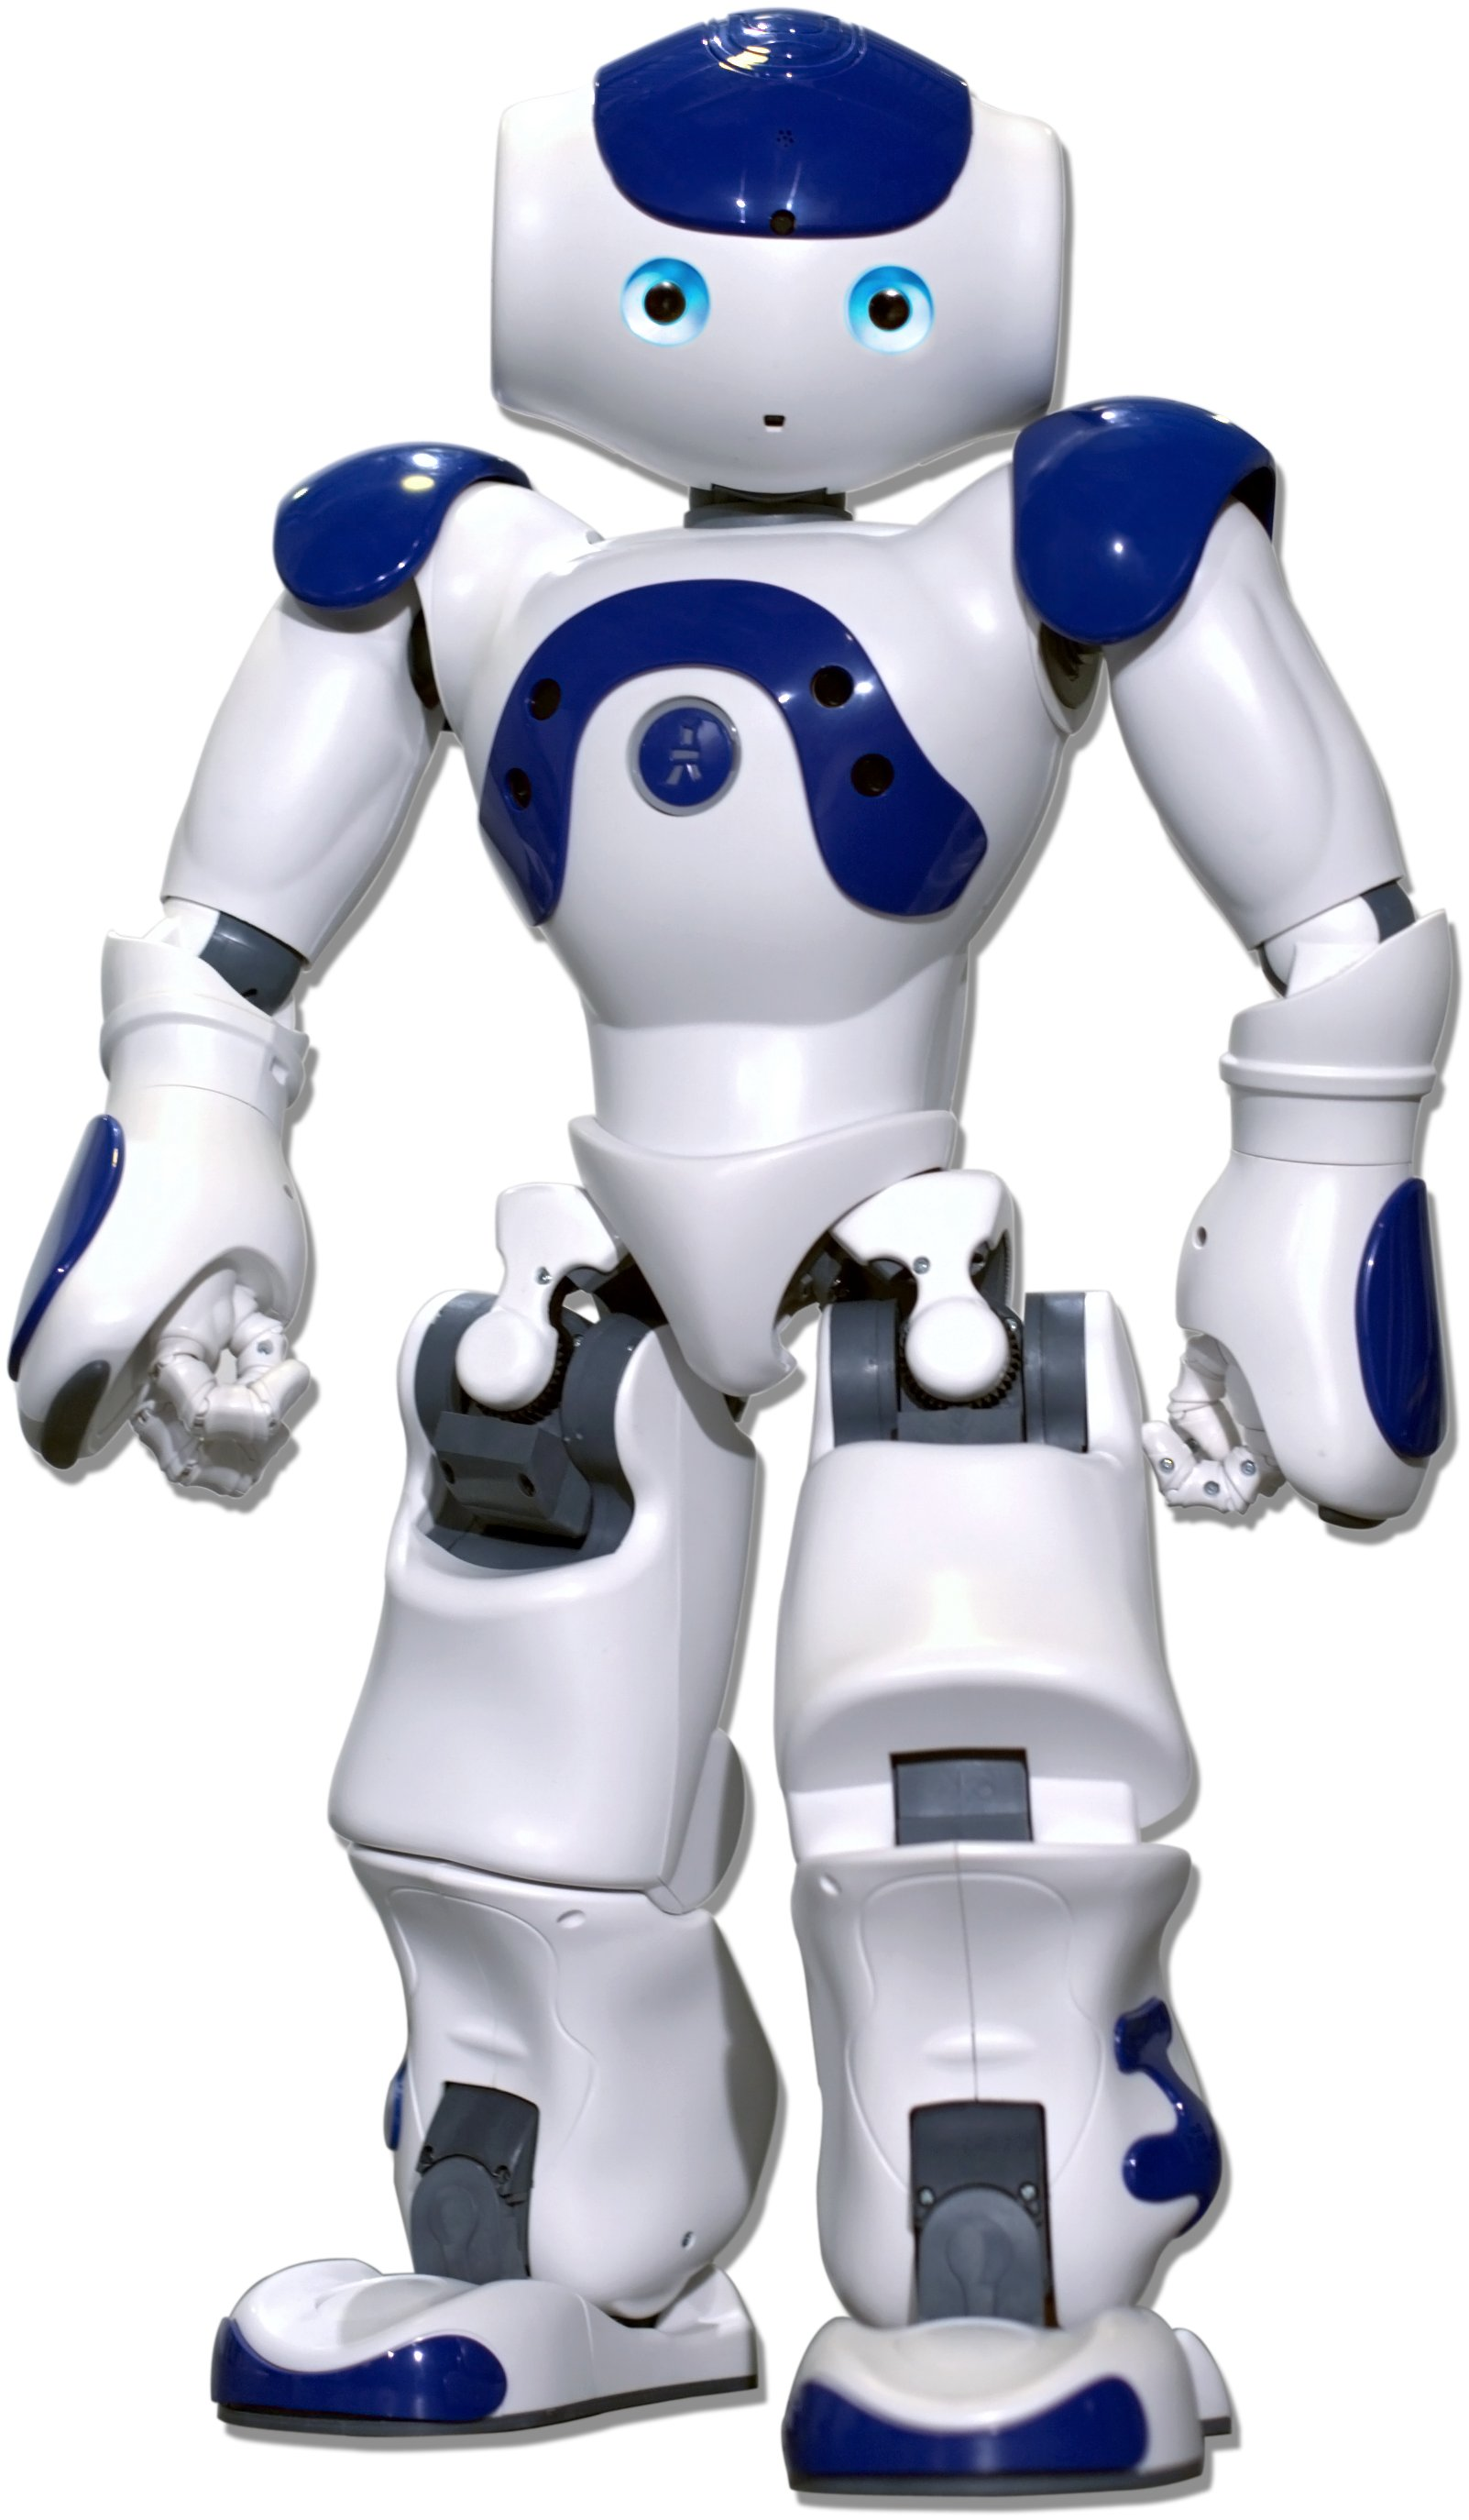
\includegraphics[scale=0.2]{nao}
  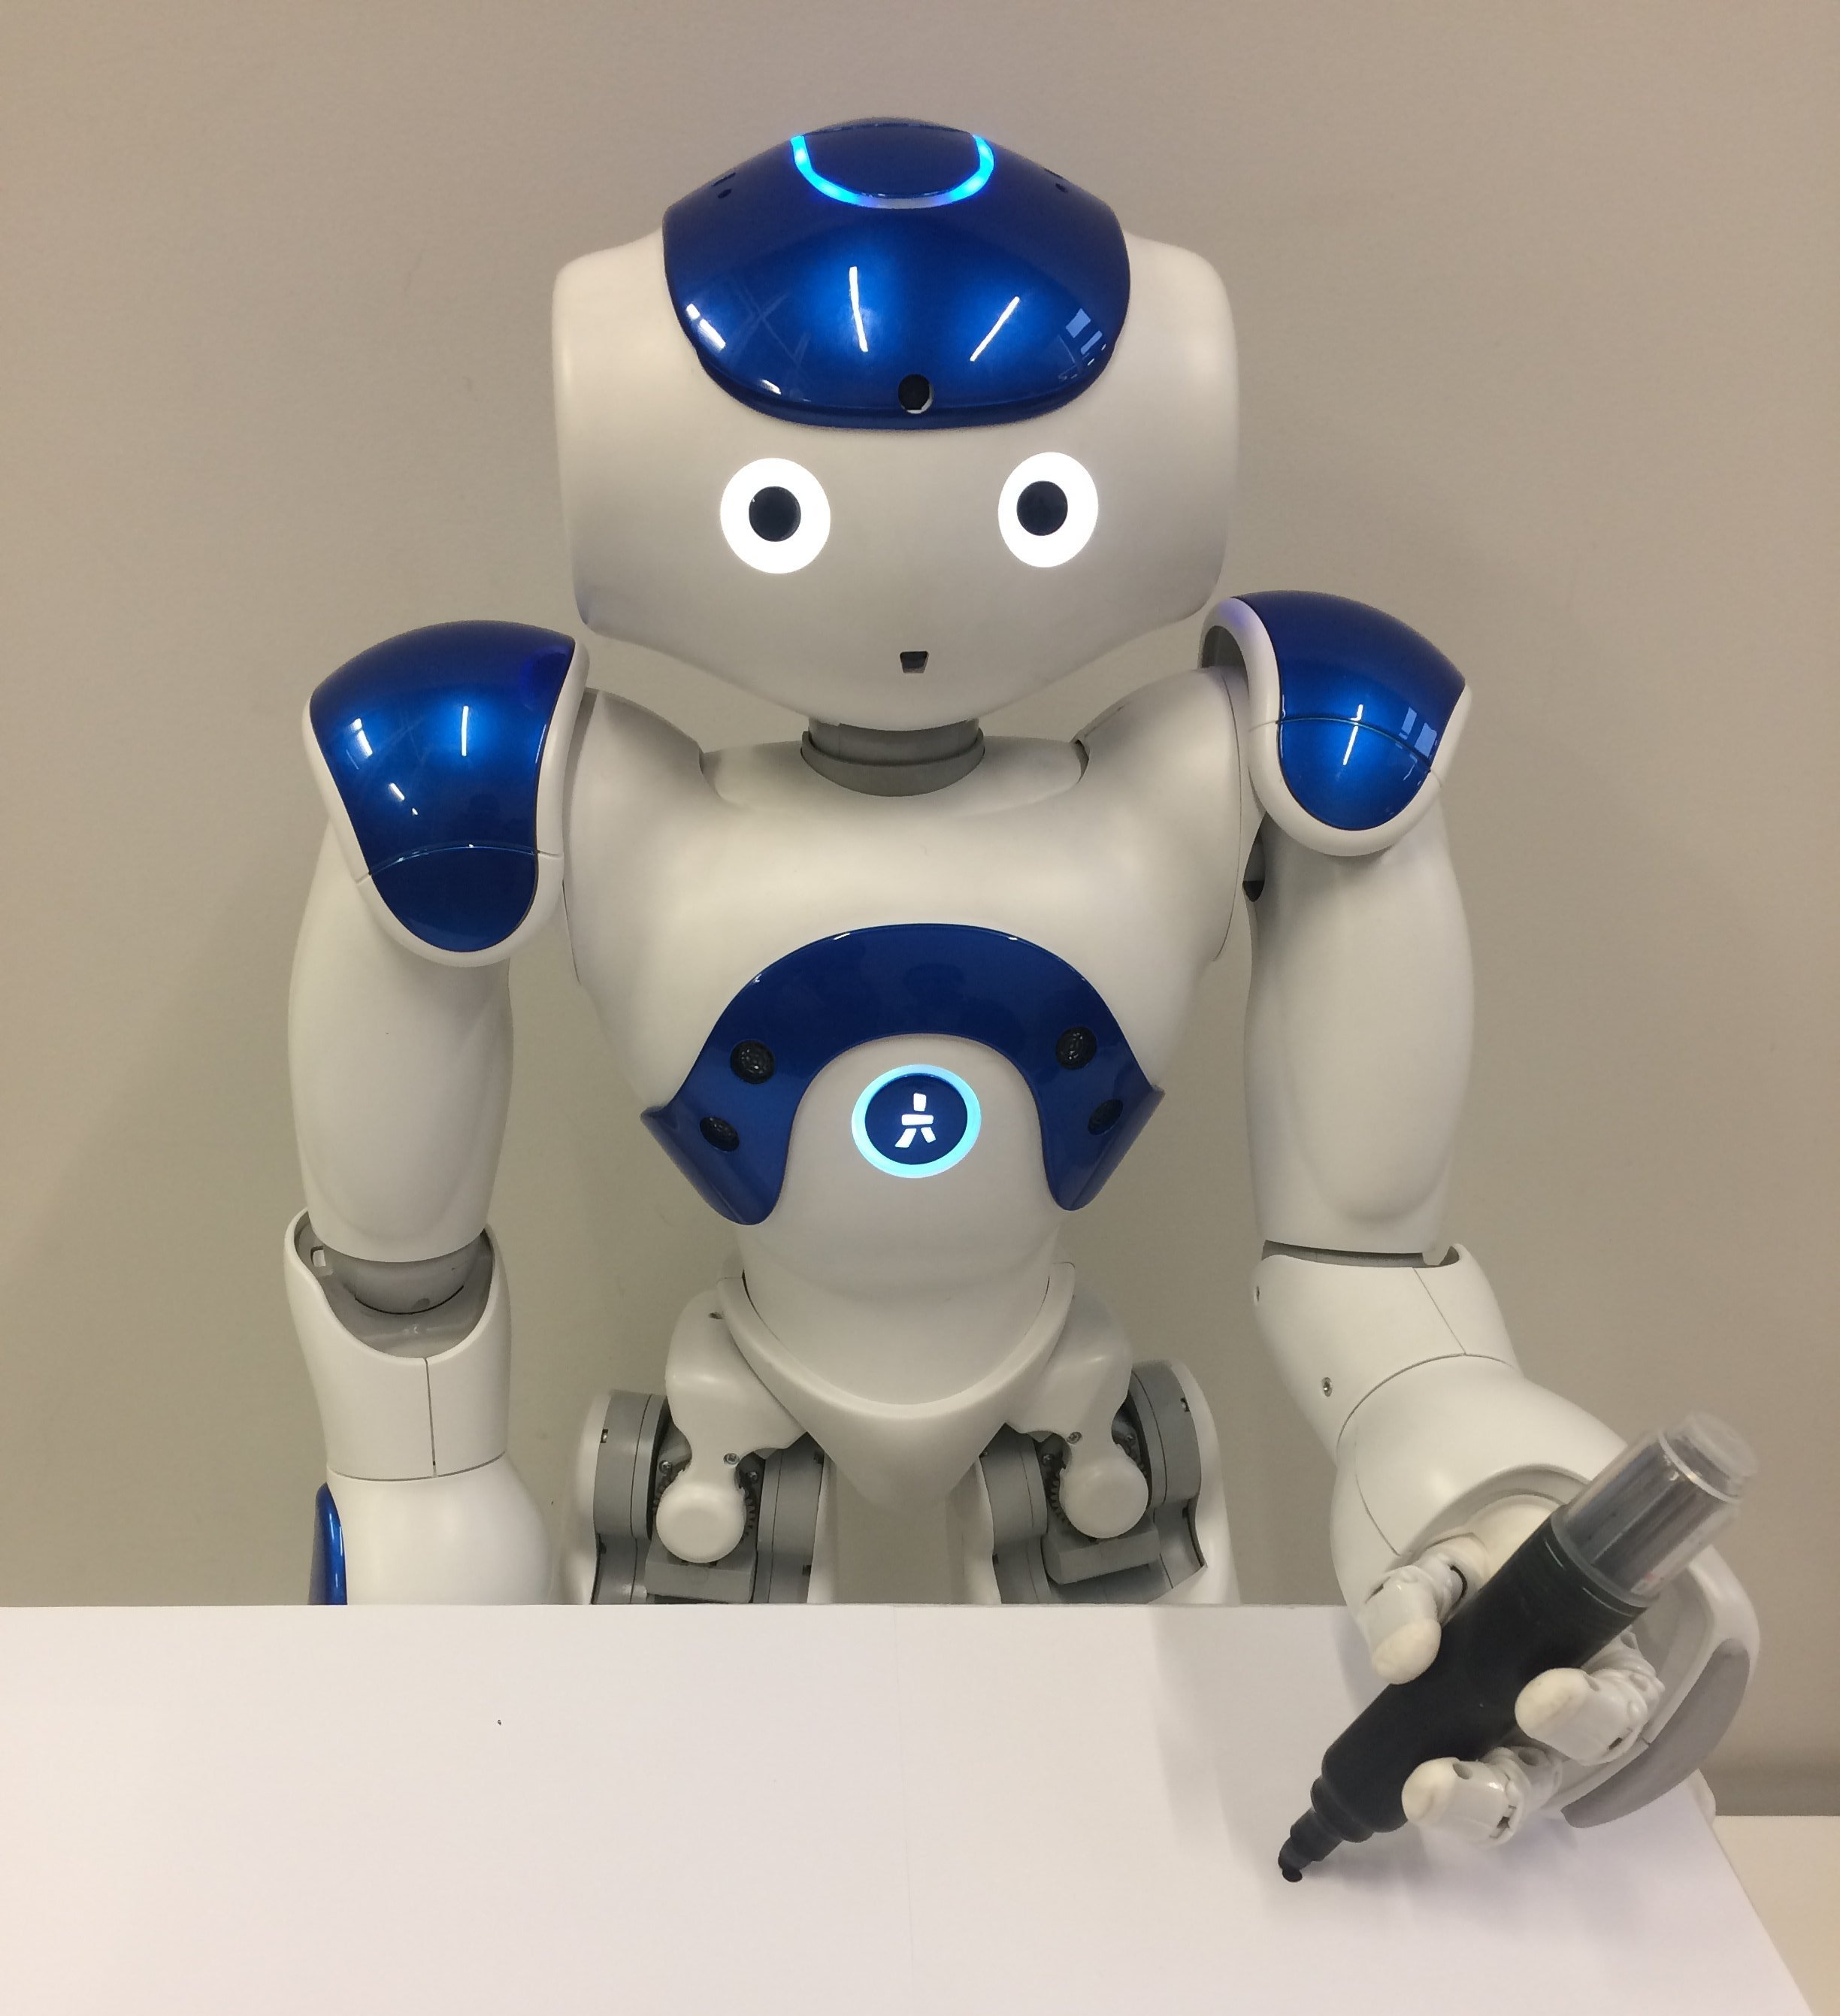
\includegraphics[width=0.3\textwidth]{nao-setup.jpg}
  %\textbf{Figure.1} NAO Humanoid Robot
  % \end{center}
  \caption{NAO Robot setup for drawing}
  \label{fig:nao}
\end{figure}

\section{Image Features Extraction}
\label{sec:methodology}

The NAO robot has two embedded RGB cameras which are used to obtain the desired images. However, the bare RGB images cannot be directly used to drive the robot motion, but need to be further processed to obtain a proper format. This section presents the image processing methods used to obtain the desired image features that will be used as target points for the drawing process.

\subsection{Detecting Edges on the Image}

The first step in the processing process consists in obtaining edges from the acquired image. To this end, the RGB image needs to be converted to gray scale reducing the three channels to only one, but keeping the main image characteristics. The gray scale image contains a lot of detail and too many features that cannot be properly handled by the controller of the robot hand, and therefore needs to be simplified. This simplification, which will be useful for drawing, consists in extracting the edges of the image.

%\subsection{Canny edge detector}
To extract the edges, the Canny edge detector was used rather than other simpler edge detectors since it allows for more control over the extracted features. In general, it can provide good edge detection, good location and minimum response according to the chosen threshold parameters. The first step in the implementation consists in filtering the image with the first derivative of a Gaussian, followed by finding the intensity of the gradients and applying non-maximum suppression. Potential edges are then obtained by applying a double threshold and hysteresis.
% The Canny edge detector is an algorithm that is used to detect a wide range of edges in images. This algorithm is computationally eficient and is quite used for its good edge detection, good location and its minimum response.
% The first stage to use Canny, is to use a filter based on the first derivative of a Gaussian to be able to reduce as much noise as possible. The result is a slightly blurred image compared to the original version.
% The second step is to find the intensity of the gradient of the image; the edge of an image can point in different directions, so Canny's algorithm uses four filters to detect horizontal,vertical and diagonals edges of the blurred image. The edge detection operator (Roberts, Prewitt, Sobel) returns a value for the first derivative in the horizontal direction $(G_{y})$ and the vertical direction $(G_{x})$. From this, the edge gradient and the direction can be determined:
% \begin{equation}
% G = \sqrt{G_{x}^{2} + G_{y}^2}
% \end{equation}
% \begin{equation}
% \Theta = \arctan(G_{y}/G_{x})
% \end{equation}

After extracting the edges, spurious remaining noise needs to be eliminated and some edges might need to be enhanced. To this end, morphological operations are used to increase the features quality, in general. An opening operation is first applied to eliminate small noise points that appear in the image followed by a closing operation, which tends to undo the thinning of the previous step but without recreating the eliminated noise. The specific mask is task dependent and is mainly experimentally obtained.

% A morphological operation is used to increase the number of pixels providing a better quality to the image. This operation combines two sets using the vector subtraction of set elements. Let $A$ and $B$ be sets in the Euclidean $N$-space. The erosion of $A$ by $B$, denoted by $A \ominus B$, is the set of all elements $x$ for which $x + b \in A$ for every $b \in B$.
% and is defined by:
% \begin{equation}
% \begin{split}
% A \ominus B = &\{
% x \in E^{N} \mid x + b \in  \textrm{A for every b}  \in B, \textrm{there exists an}\\
% & \textrm{a} \in \textrm{A such that} x = a - b\}
% \end{split}
% \end{equation}
% The utility of the erosion transformation is better appreciated when the erosion is expressed in a different form. The erosion of an image $A$ by a structuring element $B$ is the set of all elements $x$ of $E^{N}$ for which $B$ translated to $x$ is contained in $A$. In fact, this was the definition used for erosion by \cite{ref6}. The proof is immediate from the definition of erosion and the definition of translation.
% \begin{equation}
% A \ominus B =\{x \in E^{N} \mid (B)_{x} \subseteq A \}
% \end{equation}
% Thus the structuring element $B$ may be visualized as a probe which slides across the image $A$, testing the spatial nature of $A$ at every point. Where $B$ translated to $x$ can be contained in $A$ (by placing the origin of $B$ at $x$), then $x$ belongs to the erosion $A \ominus B$.
% Other proposition about erosion of an image A by structuring element B is the intersection af all translations of A by the points $-b$, where $b \in B$.
% \begin{equation}
% A \ominus B = \bigcap_{b \in B} (A)_{-b}
% \end{equation}

\subsection{Topological Skeleton}

After the morphological processing, and due to the nature of the image which is arbitrary, the edges can still have a width of more than one pixel. It is necessary to have one-pixel width since these points will be provided as target points for the robot hand motion. Because of this, a topological skeletonization was implemented, which takes the morphological output as input and outputs a single pixel edge. This skeleton is a thin version of the shape and is equidistant to its boundaries, keeping the geometrical and topological properties of the obtained shapes.

After the skeleton is obtained, an initial point in the skeleton is randomly chosen and its pixel coordinates $(x_o, y_o)$ are stored. This pixel is labeled as visited. Then the neighbors of the point are checked in a given direction (e.g. to the right) to determine the next coordinate point. The coordinates of this neighbor are stored as $(x_1,y_1)$ and the pixel is labeled as visited. Once the sequence is closed, that is, the next neighbor is an already visited neighbor, or when no more neighbors are found, there will be a sequence of points $(x_i,y_i)$ which describe the target points in the image frame. Then, another non visited point in the image is chosen and the process is repeated, to generate as many continuous edges as possible.

An important remark is that skeletonizing can add some additional noise to the image, such as single pixels appearing in some parts. To reduce this noise, connectivity is checked. Elements that have less than a given (small) threshold number of pixels are removed since they are considered to be noise.

% \subsection{Hough Line Transform}
% The Hough transform is used to detect edges more precisely. For this paper will be used to detect the lines. In the space of the image, the line can be represented by the equation:
% \begin{equation}
% y = m \times x + n
% \end{equation}
% and can be plotted for each pair $(x,y)$ of the image. In this algorithm, the main idea is consider the characteristics of a line in terms of its parameters $(m,n)$, and not as points of the image $(x_{1},y_{1}),\ldots,(x_{n},y_{n})$.Based on the above, the straight line $y = m \times x + n$ can be represented as a point $(m,n)$ in the parameter space. However, when vertical lines are present, the parameters of the line $(m,n)$ are indefinite. For this reason its better to use the parameters that describe a line in polar coordinates, denoted $(\rho, \theta)$. The parameter $\rho$ represents the distance between the origin of coordinates and the point $(x,y)$, while $\theta$ is the angle of the vector of the line perpendicular to the original line and passing through the coordinate origin. Using this parameterization, the equation of a line can be written as follows:
% \begin{equation}
% \label{1}
% y = (\frac{-\cos\theta}{\sin\theta})\times x + (\frac{\rho}{\sin\theta})
% \end{equation}
% where the equation (\ref{1}) could be rewrite as:
% \begin{equation}
% \label{2}
% \rho = x \times \cos\theta + y \times \sin\theta
% \end{equation}

% Then, it is possible to associate to each line a pair $(\rho,\theta)$ that is unique if $\theta \in [0,\pi)$ and $\rho \in \textbf{R}$ or $ \theta \in [0,2*\pi)$ and $\rho \geq 0$.The space $(\rho,\theta)$ is called the Hough space for the set lines in two dimensions. For an arbitrary point in the image with coordinates $(x_{0},y_{0})$, the lines passing through that point are the pairs $(\rho,\theta)$, in equation (\ref{2}) where $\rho$ (the distance between the straight line and the origin) is determined by $\theta$. This corresponds to a sinusoidal curve in space $(\rho,\theta)$, which is unique for that point. If the curves corresponding to two points intersect, the point of intersection in the Hough space corresponds to a line in the space of the image that passes through these two points. Generalizing, a set of points that form a line, will produce sinusoids that intersect in the parameters of that line.

\subsection{System Calibration}

The points $(x_i,y_i)$ obtained in the previous steps are given with respect to the image frame and in pixels. However, the robot needs 3D Cartesian coordinates given in its own reference frame (typically with respect to its torso). To convert from the image frame to the robot frame, the corners of the image are identified with a predefined workspace where the robot should draw. These 3D workspace corners are known values measured with respect to the robot reference frame. The ratio between the width and height of the rectangular 3D workspace, and the width and height (in pixels) of the image itself is used to scale the pixels adjusting them to the 3D world. The image plane is then fitted to the 3D workspace plane as such, keeping the height of the plane constant. These new 3D coordinates will be referred to as $\x_{des} = (x_d, y_d, z_d)$ where $z_d$ is constant.

\section{Robot Motion Generation}

After extracting the image features from the shown design, a set of desired points are given to the robot for it to follow. As previously mentioned, these points are close enough to guide the robot properly over the drawing surface, since a position-controlled scheme is used and there is no force feedback or arm compliance. Due to this structural restriction, the proper selection of the target points is critical. However, once they are properly chosen, the control scheme tracks them in Cartesian space avoiding motion discontinuities due to the differential method of the approach.

\subsection{Differential Kinematics Scheme}

The robot can move either the right or the left arm for reproducing the shown object by following the prescribed points in Cartesian space. To generate its motion, a differential scheme is used. Let $\x$ be the Cartesian position of the robot end-effector (i.e. its hand), and $\q$ be the vector containing the joint configuration. The forward kinematics of the end effector is given by
\begin{equation}
  \label{eq:forward-kine}
  \x = \f(\q)
\end{equation}
where $\f$ is the forward kinematics function and contains highly nonlinear terms. These nonlinear terms make it complicated to obtain a closed form solution. Some analytic solutions to this problem exist for specific robots, such as the NAO arm \cite{}, but they cannot be generalized, and are robot dependent. Moreover, it is sometimes not easy to automatically choose among all the possible solutions.

Rather than obtaining the analytical solution, this work uses a differential kinematics approach since it is easily generalized to any type of robot once the forward kinematics is known (considering the ease of obtaining the forward kinematics using the Denavit-Hartenberg parameters or specialized libraries that parse the robot model). The differential approach provides the following relation between Cartesian space velocities $\dot{\x}$ and joint velocities $\dot\q$:
\begin{equation}
  \dot\x = J \dot\q
\end{equation}
where $J=\frac{\partial \x}{\partial \q}$ is the end-effector Jacobian. This relation is linear an can be inverted as
\begin{equation}
  \label{eq:dot-q}
  \dot\q = J^{\#} \dot \x
\end{equation}
where $J^{\#}$ denotes the pseudo-inverse of the Jacobian. This work uses the Moore-Penrose pseudo-inverse. In \eqref{eq:dot-q} The pseudo-inverse is used instead of the inverse since $J$ is not always an invertible matrix, and is usually not even an square matrix. When the robot is close to a singularity, which can be checked by continuously monitoring the rank of $J$, a damped least-squares solution is used to avoid large joint velocities.


\subsection{Cartesian Space Reference}

The desired points are provided in the Cartesian space whereas the differential scheme \eqref{eq:dot-q} uses $\dot\x$. To include the Cartesian information in terms of the velocity, an error needs to be first defined as
\begin{equation}
  \label{eq:2}
  \e = \x - \x_{des}
\end{equation}
where $\x_{des}$ is the desired Cartesian position and $\x$ is the current position obtained from the current joint configuration with forward kinematics using \eqref{eq:forward-kine}. Considering constant desired points, the derivative of the error is $\dot\e = \dot\x$ and therefore \eqref{eq:dot-q} can be rewritten as
\begin{equation}
  \label{eq:eq-dqe}
  \dot\q = J^{\#} \dot \e
\end{equation}
which considers the joint velocities in terms of the variation of the Cartesian error. This variation can now be chosen so as to make the error decrease monotonically to zero as
\begin{equation}
  \label{eq:de-ref}
  \dot\e^{*} = -\lambda \e
\end{equation}
where $\lambda>0$ is a real value that guarantees exponential convergence of the error to zero. Then, this error reference \eqref{eq:de-ref} is applied to \eqref{eq:eq-dqe} to obtain the desired joint motion.

The final step consists in obtaining the joint positions from the joint velocities. Consider the joint configuration at time $k$ to be $\q_k$, and the joint velocity to be $\dot \q_k$. The joint configuration at time $k+1$ is obtained as
\begin{equation}
  \label{eq:Euler}
  \q_{k+1} = \q_k + \Delta T \dot\q_k
\end{equation}
where $\Delta T$ is the control time. This control time depends on each specific robot but is typically less than $10$ ms. Due to the fast control time, the integration scheme shown in \eqref{eq:Euler} is usually a good approximation to the real joint configuration. If a slower control time was to be used, another integration method would need to be used such as a Runge-Kutta integration, but this is not usual in practice.


% \subsection{Right Hand Inverse Kinematics}
% Being a humanoid, the 'extremities' of the robot can be recognized, each, as independent kinematic chains. Each of these systems allows the accomplishment of different basic tasks such as standing, walking, sitting, among others. To have control over such tasks, it is necessary to know the inverse kinematics of each kinematic chain. Due to the activity in which we focus on this work, it is necessary to perform only the inverse kinematics of the kinematic chain corresponding to the right hand of the robot. Thus, we begin by defining the transformation matrix $T$:

% \begin{equation}
% T= 
% \begin{pmatrix}
% 	r_{11}	& r_{12}	& r_{13}	&r_{14}\\
% 	r_{21}	& r_{22}	& r_{23}	&r_{24}\\
% 	r_{31}	& r_{32}	& r_{33}	&r_{34}\\
% 	0		& 0			& 0			& 1
% \end{pmatrix}
% \end{equation}

% \begin{strip}
% \begin{equation}
% r_{11} = sin(\theta_{4})(sin(\theta_{1})sin(\hat{\theta_{3}})-cos(\theta_{1})cos(\hat{\theta_{2}})cos(\hat{\theta_{3}}))-cos(\theta_{1})cos(\theta_{4})sin(\hat{\theta_{2}})
% \end{equation}

% \begin{equation}
% r_{12} = cos(\theta_{4})(sin(\theta_{1})sin(\hat{\theta_{3}})- cos(\theta_{1})cos(\hat{\theta_{2}})cos(\hat{\theta_{3}}))+ cos(\theta_{1})sin(\theta_{4})sin(\hat{\theta_{2}})\\
% \end{equation}
% \begin{equation}
% r_{13} = cos(\hat{\theta_{3}})sin(\theta_{1})+cos(\theta_{1})-cos(\hat{\theta_{2}}sin(\hat{\theta_{3}}))\\
% \end{equation}
% \begin{equation}
% r_{14} = l_{4}( sin(\theta_{4})( sin(\theta_{1})sin(\hat{\theta_{3}})- cos(\theta_{1})cos(\hat{\theta_{2}})cos(\hat{\theta_{3}}) ) )\\
% \end{equation}
% \begin{equation}
% r_{21} = cos(\hat{\theta_{2}})cos(\theta_{4})- cos(\hat{\theta_{3}})sin(\hat{\theta_{2}})sin(\theta_{4})\\
% \end{equation}
% \begin{equation}
% r_{22} = cos(\hat{\theta_{2}})sin(\theta_{4})- cos(\hat{\theta_{3}})sin(\hat{\theta_{2}})cos(\theta_{4})\\
% \end{equation}
% \begin{equation}
% r_{23} = sin(\hat{\theta_{2}})sin(\hat{\theta_{3}})\\
% \end{equation}
% \begin{equation}
% r_{24} = l_{1}+ l_{3}cos(\hat{\theta_{2}})+ l_{4}(cos(\hat{\theta_{2}})cos(\theta_{4})- cos(\hat{\theta_{3}})sin(\hat{\theta_{2}})sin(\theta_{4}))\\
% \end{equation}
% \begin{equation}
% r_{31} = sin(\theta_{4})(  cos(\theta_{1})sin(\hat{\theta_{3}})+ cos(\hat{\theta_{2}})cos(\hat{\theta_{3}})sin(\theta_{1}))+ cos(\theta_{4})sin(\theta_{1})sin(\hat{\theta_{2}})\\
% \end{equation}

% \begin{equation}
% r_{32} = cos(\theta_{4})(  cos(\theta_{1})sin(\hat{\theta_{3}})+ cos(\hat{\theta_{2}})cos(\hat{\theta_{3}})sin(\theta_{1}))- sin(\theta_{4})sin(\theta_{1})sin(\hat{\theta_{2}})\\
% \end{equation}
% \begin{equation}
% r_{33} = cos(\theta_{1})cos(\hat{\theta_{3}})- cos(\hat{\theta_{2}})sin(\theta_1)sin(\hat{\theta_{3}})\\
% \end{equation}

% \begin{equation}
% r_{34} = l_{2}+ l_{4}( sin(\theta_{4})(  cos(\theta_{1})sin(\hat{\theta_{3}})+cos(\hat{\theta_{2}})cos(\hat{\theta_{3}})sin(\theta_{1})  )+ cos(\theta_{4})sin(\theta_{1})sin(\hat{\theta_{2}})   )+ l_{3}sin(\theta_{1})sin(\hat{\theta_{2}})\\
% \end{equation}
% \end{strip}

% \begin{strip}
% where $\hat{\theta_{2}}$ represents the second joint. From this, due to the symmetry of both arms, we can define inverse kinetics as:
% \end{strip}
% \begin{strip}
% \begin{equation}
% \theta_{1}= \pm acos(\frac{T'_{(3,3)}+ \frac{T'_{(1,3)}sin(-\theta_{3})cos(\theta_{2}-\frac{pi}{2})}{cos(-\theta_{3})}}{cos(-\theta_{3})+ \frac{(cos(\theta_{2}-\frac{pi}{2}))^2(sin(-\theta_{3}))^2}{cos(-\theta_{3})}})\\
% \end{equation}
% \end{strip}
% \begin{strip}
% \begin{equation}
% \theta_{1}= \pm acos(\frac{T'_{(1,3)}}{cos(\theta_{2}-\frac{\pi}{2})sin(-\theta_{3})})\\
% \end{equation}
% \end{strip}
% \begin{strip}
% \begin{equation}
% \theta_{2}= \pm acos(\frac{T'_{(2,4)}-l_{1}-(\frac{l_{4}sin(\theta_{4})T'_{(2,2)}}{\cos(\theta_{4})})}{l_{3}+l_{4}cos(\theta_{4})+l_{4}\frac{(sin(\theta_{4}))^2}{cos(\theta_{4})}})\\
% \end{equation}
% \end{strip}
% \begin{strip}
% \begin{equation}
% \theta_{3}= -asin(\frac{T'_{(2,3)}}{sin(\theta_{2}-\frac{\pi}{2})})\\
% \end{equation}
% \end{strip}
% \begin{strip}
% \begin{equation}
% \theta_{3}= (\pi-asin(\frac{T'_{(2,3)}}{sin(\theta_{2}-\frac{\pi}{2})}))\\
% \end{equation}
% \end{strip}
% \begin{strip}
% \begin{equation}
% \theta_{4}= (\pi-acos(\frac{l_{3}^2+l_{4}^2-\sqrt{(s_{x}-T'_{(1,4)})^2+(s_{y}-T'_{(2,4)})^2+(s_{z}-T'_{(3,4)})^2}^2}{2l_{3}l_{4}}))
% \end{equation}
% \end{strip}

\section{Drawing Scheme}
%\label{sec:methodology}
This section explains the steps that had to be followed to make the NAO able to obtain the points of the image to be plotted. In the (ADD FIGURE) the flow diagram is shown where the steps performed are shown in detail.
It was divided into two parts for this experimentation, the first part is to obtain the points of the image. For this part it is necessary that the user can make an example drawing, as can be seen in (ADD FIGURE) From this example the NAO should take a screenshot, with its front camera, of this image to go to the processing part from image. As you can see in (ADD FIGURE). Once the image acquisition step has been performed, the pre-processing of the image where the morphological method of Dilation and Erosion is applied is performed in order to improve the quality of the image. As can be seen in (ADD FIGURE). After this step the Canny methods were applied to detect the edges of the image (ADD FIGURE), after that realize to morphological skeleton and to obtain the points of the image. Once the part of the image processing is done and the Cartesian points of the operational space are obtained, the data is stored in a topic in ROS (Robot Operation System) and the inverse kinematics are calculated. This allows to simulate the movement of the right arm of the NAO following the trajectory of the images shown above (ADD FIGURE).

\begin{strip}
\centering
\captionsetup{font=footnotesize}
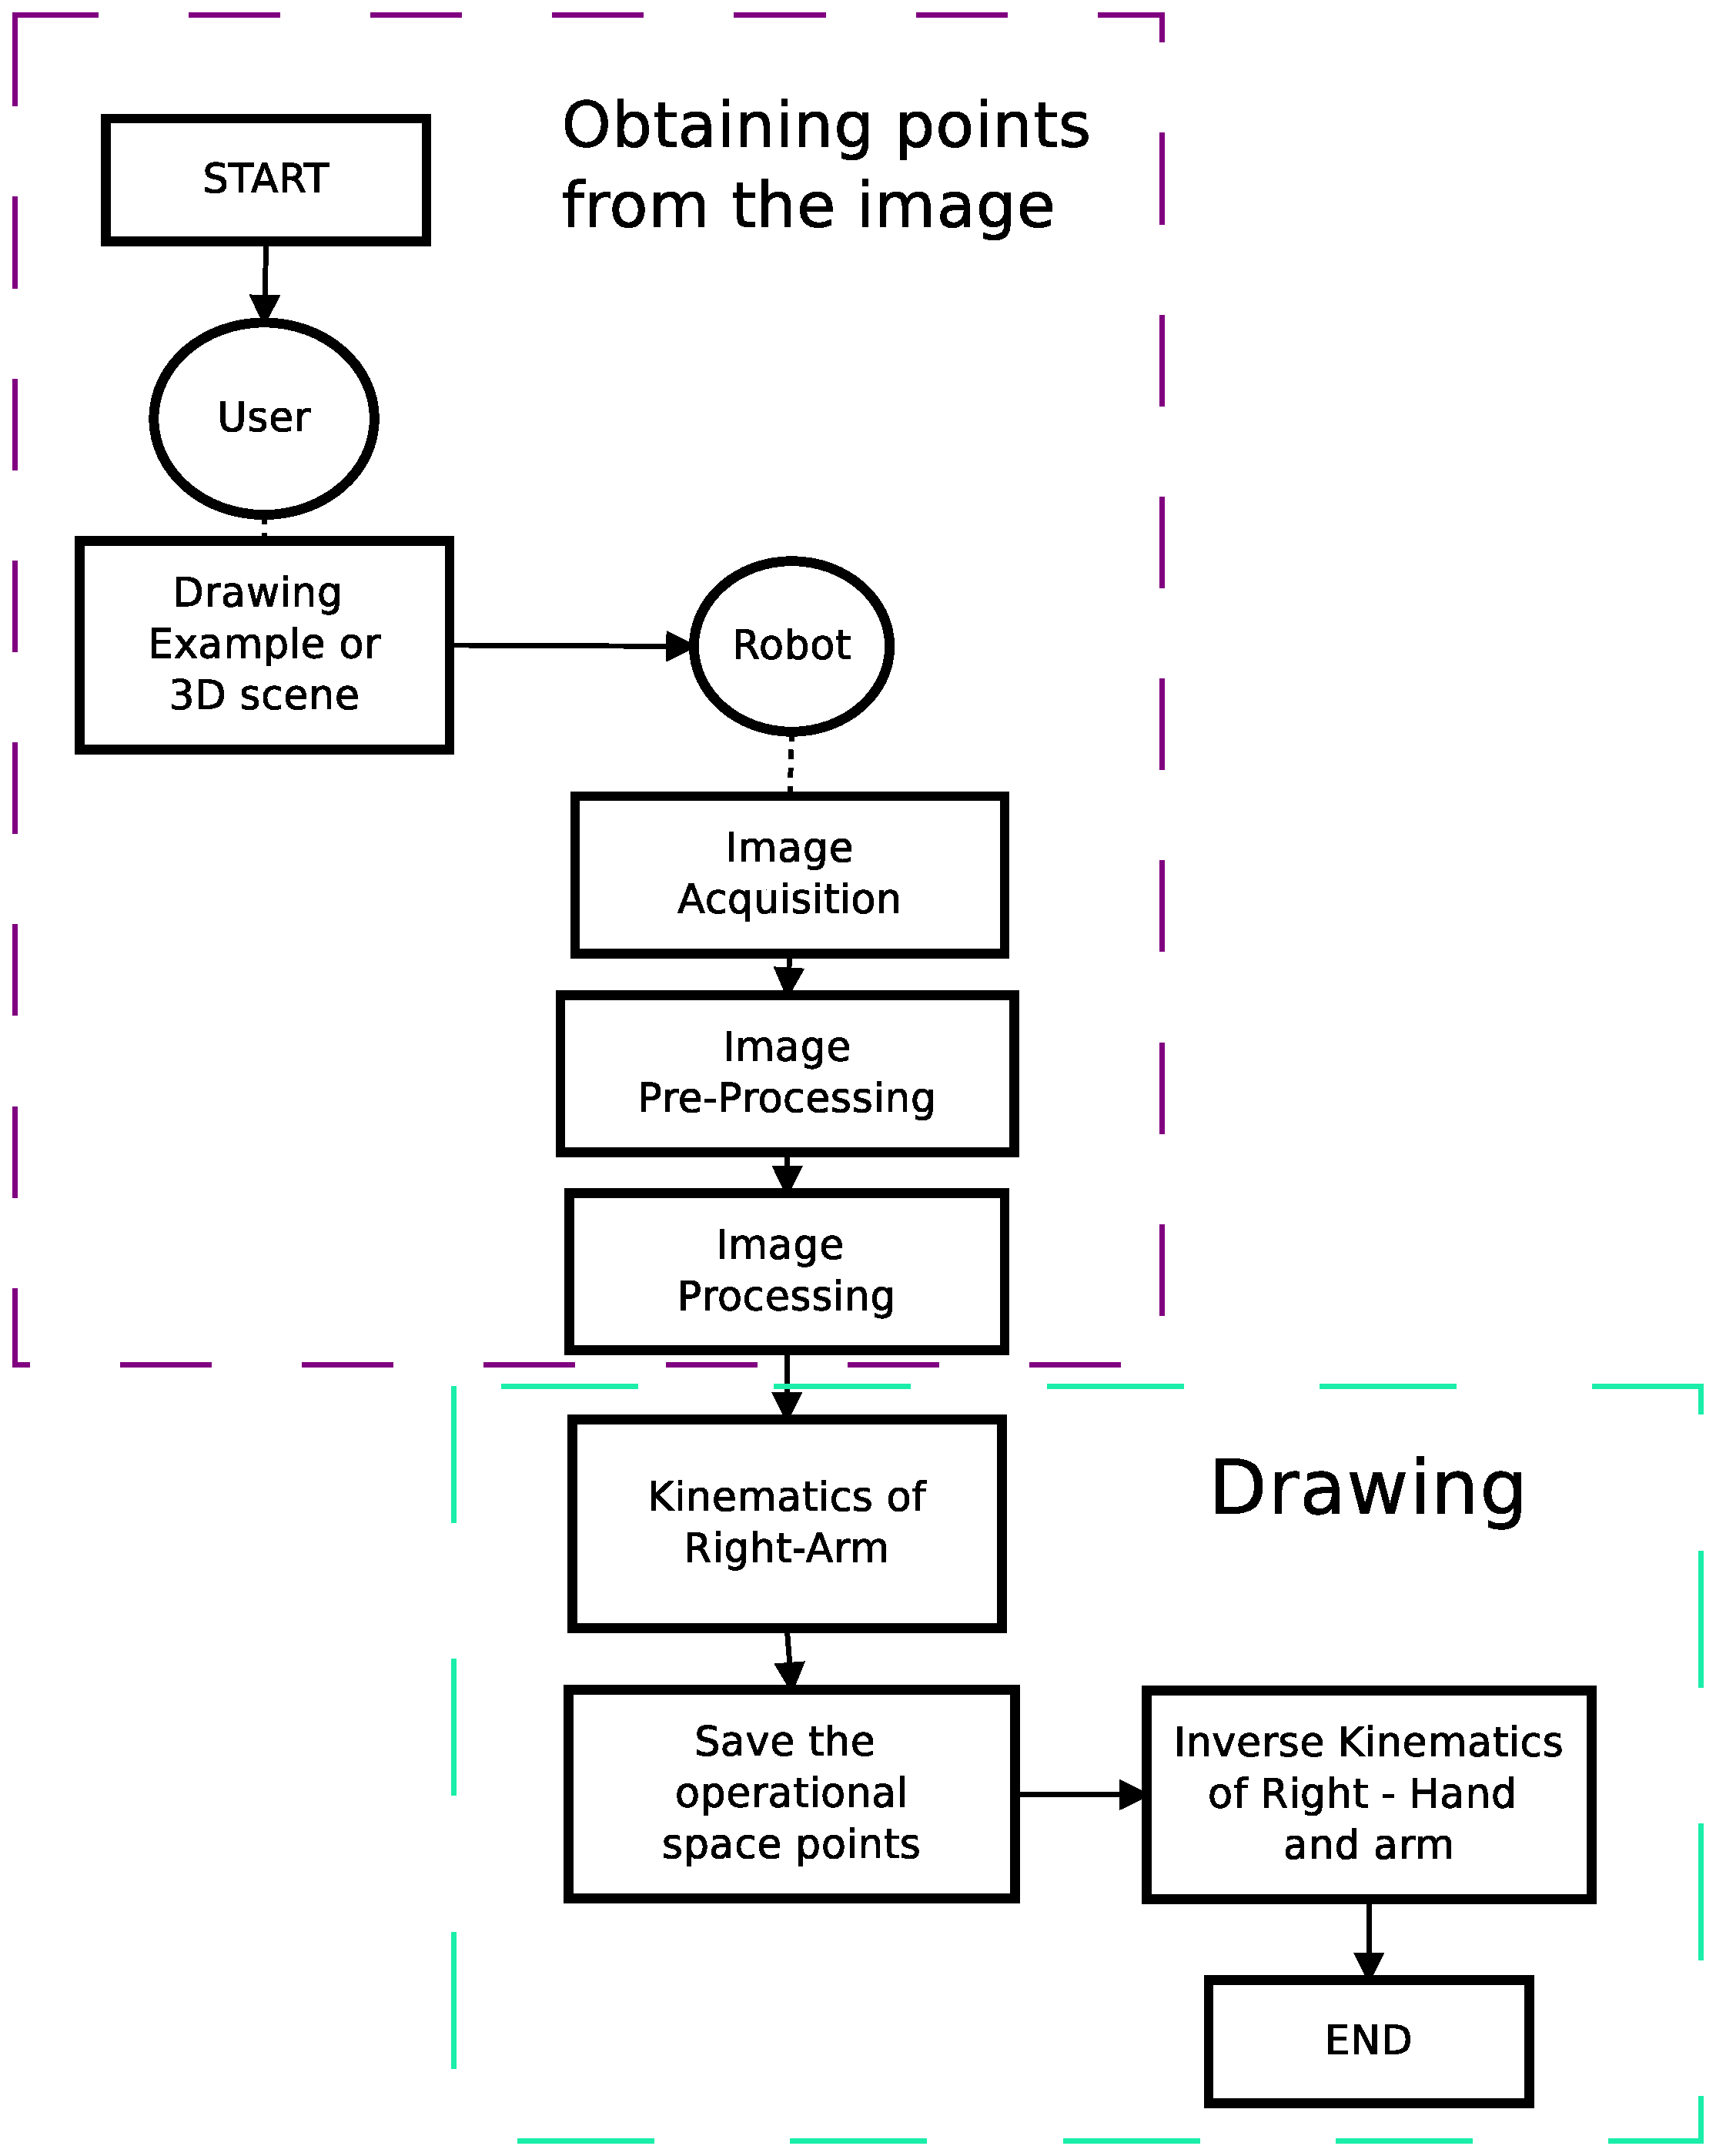
\includegraphics[width=0.6\textwidth]{flowchart.eps}\\
%\caption{Flowchart for that NAO can draw.}
\textsc{Figure 2:} Flowchart for that NAO can draw.
\end{strip}

\section{Results}

This section shows the results of the different processes that were performed on the images and then have the NAO take the coordinate points and can move the right arm according to the trajectory that originates by putting all these points together.

\begin{figure}[htb]
\centering
~\subfloat[Original Image]{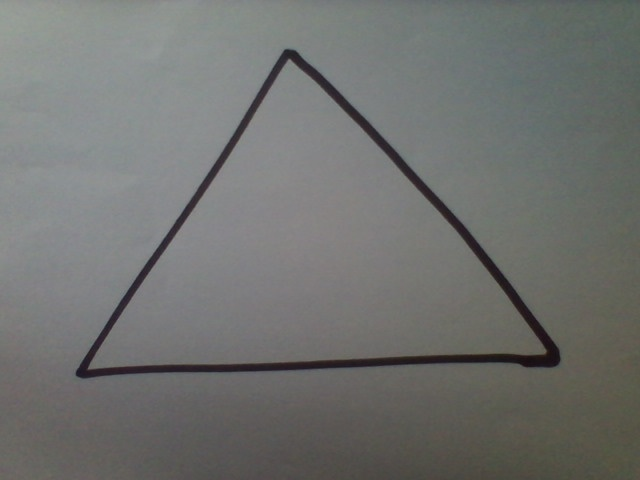
\includegraphics[width=40mm]{orig_tria.jpg}}
~\subfloat[Canny Image]{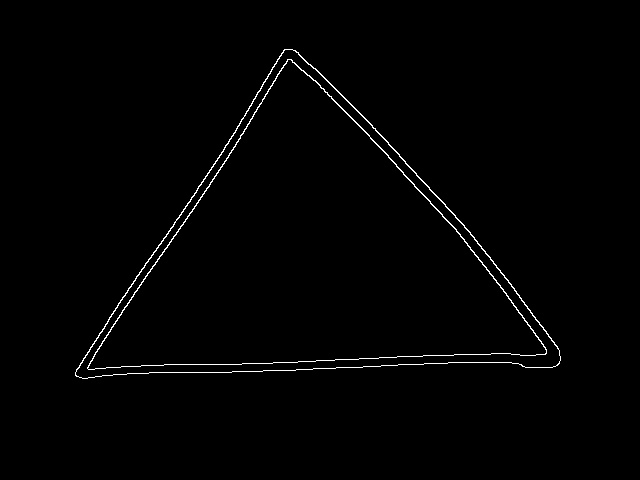
\includegraphics[width=40mm]{canny_tria.jpg}}
~\subfloat[Dilate Image]{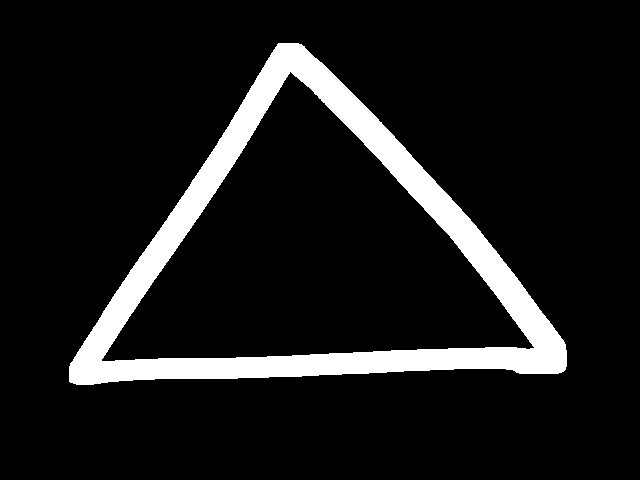
\includegraphics[width=40mm]{dilate_tria.jpg}}
~\subfloat[Erosion Image]{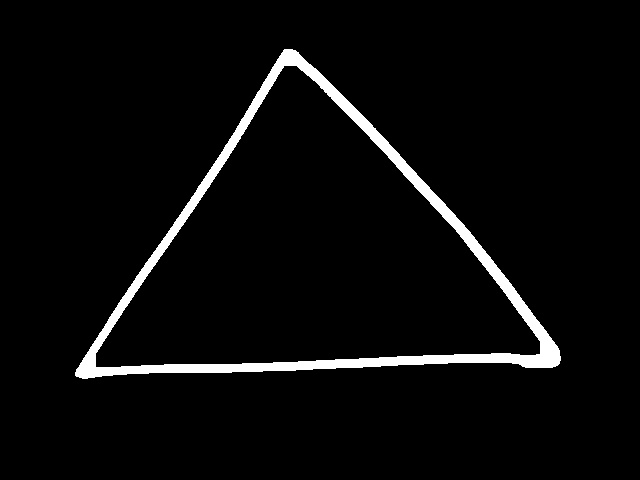
\includegraphics[width=40mm]{erode_tria.jpg}}
~\subfloat[Skeleton Image]{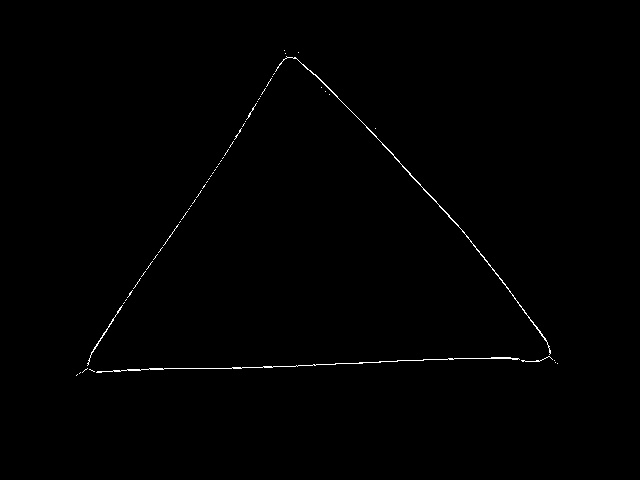
\includegraphics[width=40mm]{skel_tria.jpg}}
\caption{Steps of image processing} \label{fig:triangle}
\end{figure}


\begin{figure}[htb]
\centering
~\subfloat[Original Image]{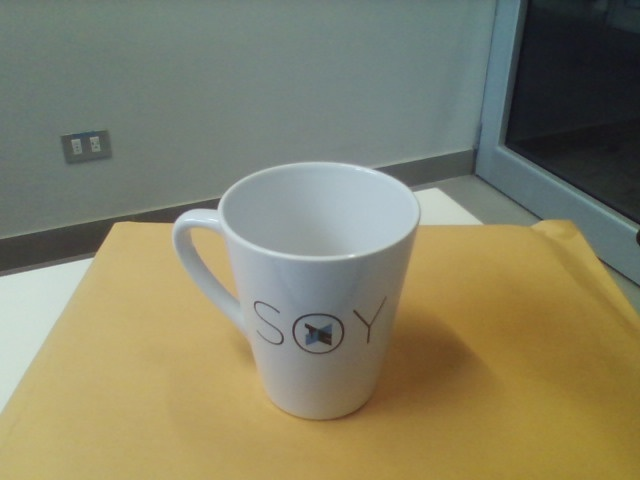
\includegraphics[width=40mm]{imagen_original.jpg}}
~\subfloat[Canny Image]{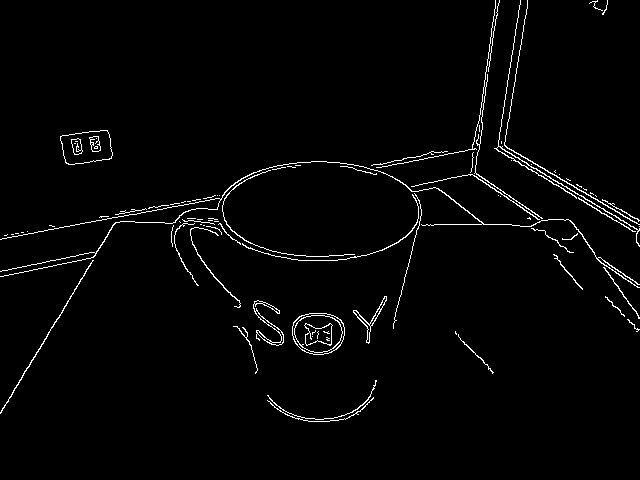
\includegraphics[width=40mm]{canny_taza.jpg}}
~\subfloat[Dilate Image]{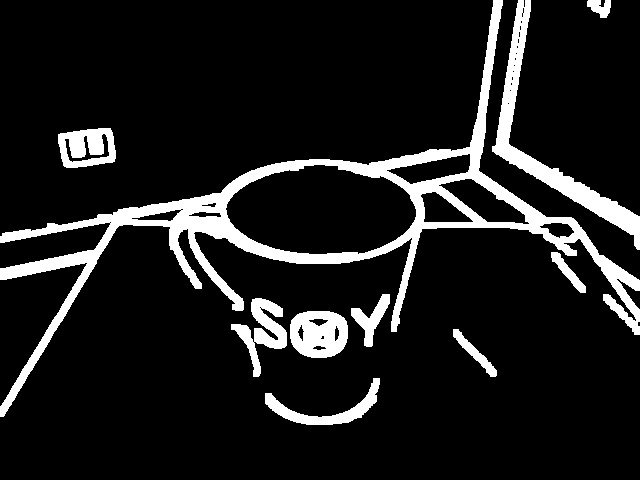
\includegraphics[width=40mm]{dilation_taza.jpg}}
~\subfloat[Erosion Image]{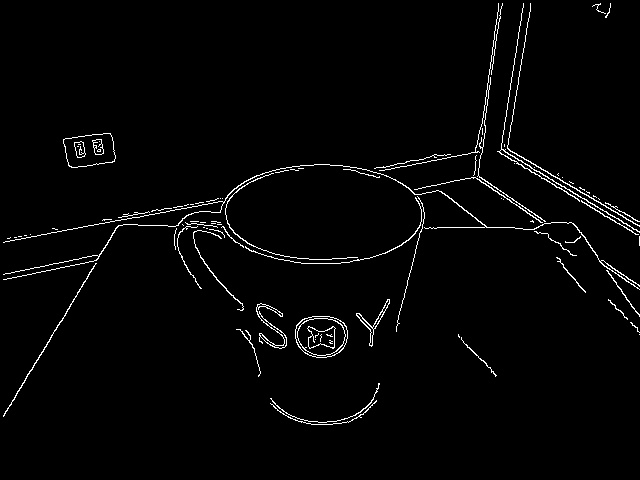
\includegraphics[width=40mm]{erode_taza.jpg}}
~\subfloat[Skeleton Image]{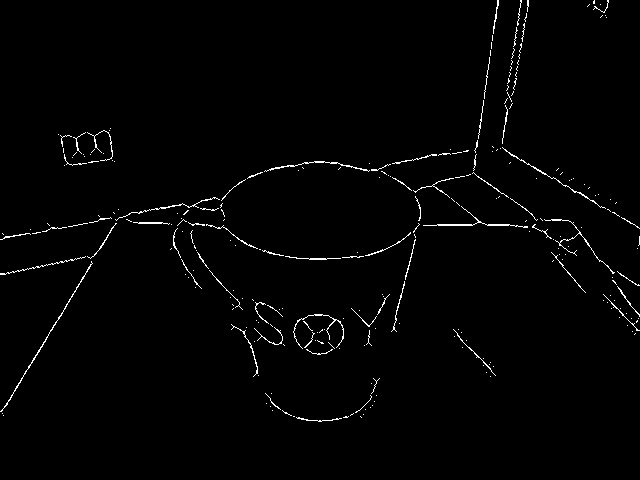
\includegraphics[width=40mm]{skel_taza.jpg}}
\caption{Steps of image processing} \label{fig:cup}
\end{figure}

\begin{figure}
\centering
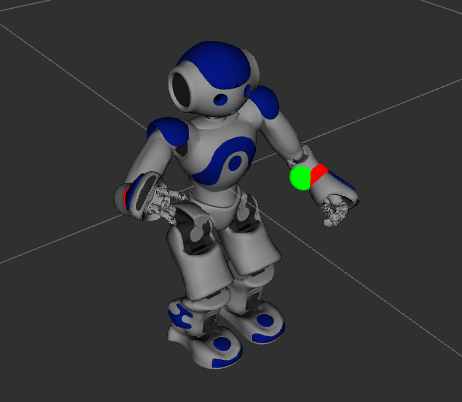
\includegraphics[scale=0.3]{nao1.png}
\caption{Simulation of the right arm of Robot NAO}
\end{figure}
\section{Conclusion}
\label{sec:conclusion}

% references section
\bibliographystyle{IEEEtran}
\bibliography{biblio.bib}
\end{document}

% Prueba
